\section{Budowa aplikacji}
\begin{figure}[H]
	\centering
	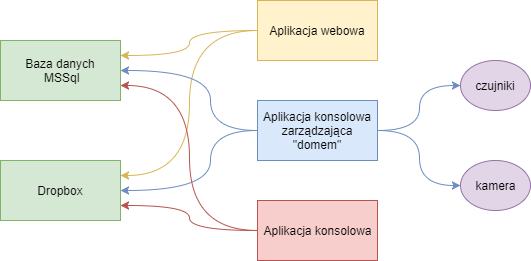
\includegraphics[scale=0.8]{schemat_systemu.png}
	\caption{Budowa systemu zarządzania domem}
	\label{fig:schemat_systemu}
\end{figure}
Aplikację powstałą na potrzeby tej pracy można podzielić na 3 moduły, które zostały przedstawione na rysunku \ref{fig:schemat_systemu}, a składają się na nie :
\begin{itemize}
\item Aplikacja webowa- interfejs pozwalający na zlecanie nowych zadań aplikacji konsolowej oraz odczyt wyników przesłanych przez nią oraz przez program zarządzający domem,
\item Aplikacja konsolowa- przetwarza zadania detekcji oraz rozpoznawania twarzy zlecone za pomocą aplikacji webowej,
\item Program zarządzający domem- przekazuje cyklicznie odczytywane dane z czujników oraz wykryte ruchy do bazy danych, w celu dalszej obróbki przez pozostałe moduły.
\end{itemize}
Na usługi pomocnicze wykorzystane w projekcie składają się
\begin{itemize}
\item baza danych- przechowywanie danych o dodanych zadaniach, wynikach, nauczonych sieciach neuronowych oraz osobach,
\item dropbox- przechowywanie większych plików- obrazów oraz nauczonych modeli sieci.
\end{itemize}

\subsection{Wzorzec projektowy MVC}
\begin{figure}[H]
	\centering
	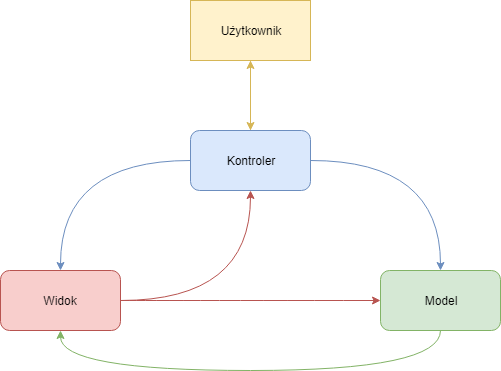
\includegraphics[scale=0.8]{mvc.png}
	\caption{Schemat klasycznego wzorca MVC}
	\label{fig:schemat_mvc}
\end{figure}
Strona internetowa powstała na bazie bardzo popularnego wśród programistów wzorca projektowego MVC. Założenia wzorca Model-Widok-Kontroler są bardzo proste, ich składowymi są:
\begin{itemize}
\item Model- reprezentuje logikę biznesową. Tutaj znajdują się wszelkie obiekty, które służą do wykonywania zaimplementowanej funkcjonalności danej aplikacji,
\item Widok- jest warstwą prezentacji. Odpowiada za prezentację logiki biznesowej (Modelu) użytkownikowi w przystępny sposób,
\item Kontroler- obsługuje żądania użytkownika. Odebrane zadania oddelegowuje do odpowiednich modeli.
\end{itemize}

\subsection{Single Page Application}
Single Page Application (SPA) to aplikacja lub strona internetowa, która w całości wczytuje się za jednym razem. Cały potrzebny do działania strony kod (HTML, CSS, JavaScript) przesyłany jest na początku lub dodawany dynamicznie w kawałkach, zwykle w odpowiedzi na interakcje generowane przez użytkownika.
Sposób działania takiej aplikacji jest zbliżony do odczuć towarzyszących korzystaniu z aplikacji desktopowej lub mobilnej.

\section{Raspberry Pi}

\section{Open Cv}

\subsection{Detekcja twarzy}
\subsubsection{Haar} \label{haar}
\subsubsection{Deep Neural Network} \label{dnn}

\subsection{Rozpoznawanie twarzy}
\subsubsection{Eigen} \label{eigen}
\subsubsection{Fisher} \label{fisher}
\subsubsection{LBPH} \label{lbph}

\section{Azure}
\subsection{Cognitive Services} \label{cognitive_services}

\section{AWS}

